\chapter{Experiments}
In this chapter, we present experimental results of our proposed methods: corpus-based translation and unsupervised translation system integrating LM and DAE. We also empirically analyze the effect of different factors in these methods. Before that, we describe the system, evaluation methodology, and datasets when the experiments are conducted.
\section{Experimental Setup}
Monoligual word embeddings have a dimensionality of 300 and  are trained as a skip-gram model using FastText (\cite{bojanowski2016enriching}) for 5 epochs, only for words that have occurs at least 10 times. (\cite{conneau2017word}). The novel corpus-based approach is also implemented on MUSE framework. Model optimization is performed with AdaM (\cite{bibid}).  Vocabulary sizes for source and target side are limited to 50k.
$5$-gram LMs are trained separately using KenLM with Kneser–Ney smoothing.\\
The training corpora for embeddings and LM are the same, containing 100M sentences respectively. Detailed statistics are in Table 6.1.\\
Context-aware translation supported is performed using beam search with beam size 10 and the best hypothesis is the one with best sentence score evaluated by LM.\\
DAE is implemented in Sockeye (\cite{hieber2017sockeye}), using RNN and Transformer architectures. RNN based DAE has 2-layer encoder and 2-layer decoder, the hidden layer size is 512.In Transfomer based DAE, encoder and decoder both have 6 layers and hidden layer size is also 512. The multi-head attention mechanism uses 6 heads. DAEs are trained on smaller corpora containing 20M sentences. \\
We evaluate the different cross-lingual embedding learning methods on word retrieval tasks. The datasets are released by \cite{conneau2017word}, which contains 12 pairs of directional dictionaries. Each dictionary contains 5000 unique words for supervised training and 1500 unique words for evaluation.  the performances of translation systems on $\texttt{newstest2016}$ German$\leftrightarrow$English task and  $\texttt{newstest2014}$ French$\leftrightarrow$English task.


\section{Corpus Statistics}
\begin{table}[H]
	\centering
	\begin{tabular}{c|c|c|c|c}
		\hline
		\multirow{4}{*}{\textbf{Train}} & \textbf{}              & \textbf{German} & \textbf{English} & \textbf{French} \\ \cline{2-5} 
		& \textbf{Sentences}     & \textbf{100M}   & \textbf{100M}    & \textbf{100M}   \\ \cline{2-5} 
		& \textbf{Running Words} & \textbf{1880M}  & \textbf{2360M}   & \textbf{3017M}  \\ \cline{2-5} 
		& \textbf{Vocabulary}    & \textbf{1254k}  & \textbf{523k}    & \textbf{660k}   \\ \hline
	\end{tabular}
	\caption{Training corpora for embeddings and LM}
\end{table}

\begin{table}[H]
	\centering
	
	\begin{tabular}{c|c|c|c|c|c}
		\hline
		\multirow{7}{*}{\textbf{Test}} & \textbf{}                      & \multicolumn{2}{c|}{\textbf{\texttt{newstest2016}}}    & \multicolumn{2}{c}{\textbf{\texttt{newstest2014}}}    \\ \cline{3-6} 
		& \multicolumn{1}{l|}{\textbf{}} & \textbf{German}       & \textbf{English}      & \textbf{French}       & \textbf{English}      \\ \cline{2-6} 
		& \textbf{Sentences}             & \textbf{2999}         & \textbf{2999}         & \textbf{3003}         & \textbf{3003}         \\ \cline{2-6} 
		& \textbf{Running Words}         & \textbf{62506}        & \textbf{64619}        & \textbf{81165}        & \textbf{71290}        \\ \cline{2-6} 
		& \textbf{Vocabulary Size}       & \textbf{11978}        & \textbf{8645}         & \textbf{10899}        & \textbf{9200}         \\ \cline{2-6} 
		& \textbf{OOV Rates}             & \textbf{4116 (6.6\%)} & \textbf{1643 (2.5\%)} & \textbf{1731 (2.1\%)} & \textbf{1299 (1.8\%)} \\ \cline{2-6} 
		& \textbf{LM perplexity}         & \textbf{211.0}        & \textbf{109.6}        & \textbf{51.2}         & \textbf{84.6}         \\ \hline
		
	\end{tabular}
	\caption{Evaluation corpora for translation}
\end{table}
\section{Word Transnewsteslation}
\subsection{Baseline Experiments}
 As demonstrated in Table 6.3, CSLS performs better than other dictionary induction methods: simple nearest neighbour search (NN) and inverted softmax (ISF). So in all tables related to word retrieval task, CSLS is the default method if without any specification.

\begin{table}[H]
	\centering
	\begin{tabular}{llccc}
		\hline
		\multicolumn{2}{l}{Methods}                           & NN    & ISF   & CSLS  \\ \hline
		Supervised                    & Procrustes             & 60.37 & 63.22 & 65.38 \\ \hline
		\multirow{2}{*}{Unsupervised} & Adversarial            & 47.03 & 49.57 & 53.50 \\ \cline{2-5} 
		& Adversarial+Procrustes & 61.75 & 62.68 & 64.92 \\ \hline
	\end{tabular}
	\caption{3}
\end{table}


\subsection{Corpus-based Approach}
We run the novel corpus-based approach on a relative small corpus with 50k sentences using different learning rate schedulers. One is to start from initial learning rate, the other is to inherit the learning rate after the training on previous batch sentences. The first learning rate scheduler always performs better than the second one. We demonstrate the results for German$\rightarrow$ English and English $\rightarrow$ German with the first scheduler, also the performance of  German$\rightarrow$ English with second scheduler. These are trained on a relative small corpus with 50k sentences. In order to lift the performance of the second scheduler, we augment corpus by training two loops over the 50k corpus and extend the corpus size to 200k. The results get better but still not as good as first learning rate scheduler. 
\subsubsection{Different Learning Rate Scheduler}
The tables below show results of word retrieval accuracy for online learning of corpus-based approach, where the column represents different initial learning rate and the row represents different sentence batch size.
\begin{itemize}
	\item Start from Initial Learning Rate
%	\begin{itemize}
%		\item .
		\begin{table}[h]
			\centering
		\caption{Word translation accuracy for German$\rightarrow$English word retrieval}
			\begin{tabular}{cccccc}
				\hline
				Accuracy (\%) & 100   & 500   & 1k    & 2k    & 5k    \\ \hline
				0.01          & 1.00  & 6.01  & 24.21 & 28.37 & 42.71 \\ \hline
				0.005         & 0.85  & 5.47  & 7.71  & 17.12 & 38.78 \\ \hline
				0.001         & 1.23  & 7.32  & 14.88 & 15.34 & 27.45 \\ \hline
				0.0005        & 1.54  & 45.26 & 49.88 & 54.43 & 54.97 \\ \hline
				0.0001        & 36.23 & 58.09 & 60.14 & 60.37 & 58.67 \\ \hline
			\end{tabular}

		\end{table}
%		\item Word translation accuracy for English $\rightarrow$ German, with different initial learning rates and sentence batch sizes.
		\begin{table}[h]
			\centering
		 \caption{Word translation accuracy for English $\rightarrow$ German word retrieval}
			\begin{tabular}{cccc}
				\hline
				Accuracy (\%) & 1k   & 2k   & 5k      \\ \hline
				0.01          & 10.02  & 16.50  & 23.36 \\ \hline
				0.005       & 47.65 & 22.28 & 24.21 \\ \hline
				0.001        & 24.44 & 24.98 & 26.75 \\ \hline
				0.0005          & 54.82  & 55.67  & 48.44 \\ \hline
				0.00001        & 59.21 & 58.98 & 56.90 \\ \hline
			\end{tabular}

		\end{table}	
%
%		
%	\end{itemize}
	\item Inherit Last Learning Rate
%	\begin{itemize}
%		\item Word translation accuracy for German$\rightarrow$English with different initial learning rates and sentence batch sizes.\\
		\begin{table}[H]
			\centering
			\caption{Word translation accuracy for German$\rightarrow$English}
			\begin{tabular}{cccc}
				\hline
				Accuracy (\%) & 1k   & 2k   & 5k      \\ \hline
				0.01          & 7.79  & 4.70  & 6.01 \\ \hline
				0.005       & 3.39 & 12.03 & 8.94 \\ \hline
				0.001        & 5.40 & 11.49 & 18.89 \\ \hline
				0.0005          & 5.78  & 8.33  & 10.25 \\ \hline
				0.00001        & 51.50 & 37.63 & 15.27 \\ \hline
			\end{tabular}

		\end{table}	

Tables 6.4, 6.5, 6.6 demonstrates the performance of our online learning algorithm. In general, $1k$ is a option for sentence batch size. The embedding mappings from English to German and from German to English show close results.
However the second scheduler inheriting last learning rate works not as well as the first one. We augment training data by training 2 loops and extending the corpus to 200k sentences. The results are in Table 6.7, the sentence batch size is $1k$ and initial learning rate are set to $0.0001$, the best settings empirically.

		\begin{table}[H]
			\centering
				\caption{ Word translation accuracy for German$\rightarrow$English with different training corpus}
			\begin{tabular}{lc}
				\hline
				Train & Accuracy (\%) \\ \hline
				50k   & 51.50         \\ \hline
				50k $\times$ 2 & 55.51         \\ \hline
				200k  & 57.87         \\ \hline
			\end{tabular}
			
		\end{table}
%	\end{itemize}
\end{itemize}
Figure 6.1 demonstrates the training processes of different experimental settings, German$\rightarrow$English and English$'\rightarrow$German with the first scheduler and German$\rightarrow$ English with the second scheduler. We also conduct the corpus-based approach experiment without LM. We tune the learning rate decay separately. It turns out that without LM the accuracy will converge at a lower level. The second scheduler learns very slowly especially at the beginning stage. 
\begin{figure}[H]
	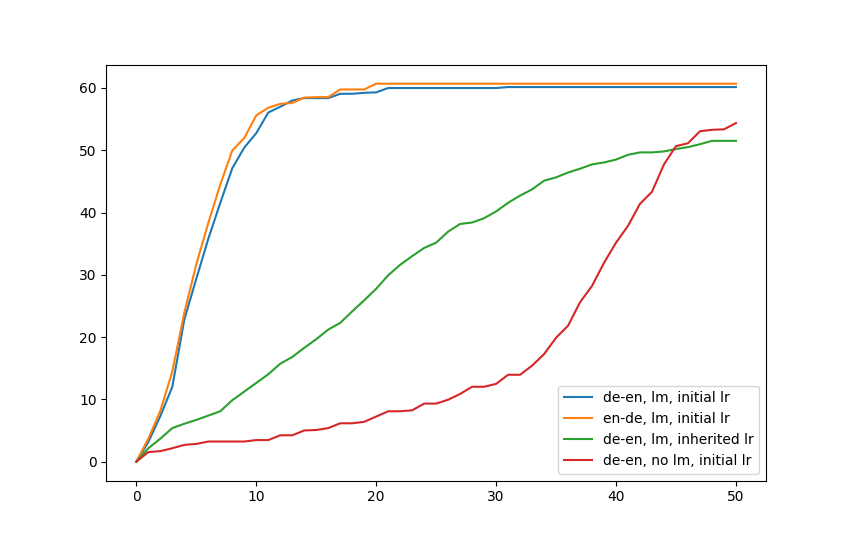
\includegraphics[width=10cm]{corpus}
	\centering
	\caption{Comparison of different experiments}
\end{figure}


\section{Sentence Translation}


\subsection{Comprehensive Table}
\begin{table}[H]
	
	\caption{Translation results on German$\leftrightarrow$English \texttt{newstest2016} and French$\leftrightarrow$English \texttt{newstest2014} }
	\centering
\scalebox{0.8}{
		\begin{tabular}{>{\bfseries}l>{\bfseries}c>{\bfseries}c>{\bfseries}c>{\bfseries}c}
			\toprule
			& De-En & En-De & Fr-En & En-Fr\\
			System   & \textsc{Bleu} [\%] & \textsc{Bleu} [\%] & \textsc{Bleu} [\%] & \textsc{Bleu} [\%]\\
			\midrule
			Word-by-Word   & 11.1 & 6.7 & 10.6 & 7.8\\
			\midrule
			+ LM (5-gram) + tgt w/ high LM score for OOV  & 12.9 & 8.9 & 12.7 & 10.0\\
			+ LM (5-gram) + copy from src for OOV		& 14.5 & 9.9 & 13.6 & 10.9\\
			\midrule
			\hspace{10pt}+ Denoising (RNN)  & 16.2 & 10.6 & 15.8 & 13.3 \\
			\hspace{10pt}+ Denoising (Transformer) & \leavevmode\color{blue}{17.2} & \leavevmode\color{blue}{11.0}& \leavevmode\color{blue}{16.5} & \leavevmode\color{blue}13.9 \\
			\midrule
			\cite{lample2017unsupervised} & 13.3 & 9.6 & 14.3 & 15.1\\
			\cite{artetxe2017unsupervised} & - & - & 15.6 & 15.1\\
			\bottomrule
		\end{tabular}

	}
\end{table}
As demonstrated above, our unsupervised MT surpass the start-of-the-art unsupervised NMT in almost all cases except English$\rightarrow$French translation. Each sub-model lift the performance respectively. Copy OOV word from source sentences works better than those predicted by language model, because OOV words are usually specific name entities and LM prefers common words rather than rare words. Denoising autoencoder based on Transformer structure outputs better translation than the traditional RNN structure. 


	\begin{table}[!h]
	\centering
	\caption {Word-by-word translation from German to English}
	\begin{tabular}{>{\bfseries}c>{\bfseries}c>{\bfseries}c}
		\hline
		&\textsc{Accuracy} [\%]& \textsc{Bleu} [\%] \\ \hline
		5M & 44.9  & 9.7  \\ \hline
		10M & 51.6 & 10.1 \\ \hline
		50M & 59.4 & 10.8 \\ \hline
		100M &\leavevmode\color{blue}61.2 & \leavevmode\color{blue}11.2 \\ \hline
	\end{tabular}
\end{table}
As in Table 6.9, larger corpus improves the word translation accuracy as well as the word-by-word translation. 

\subsection{BPE vs Word}
Byte pair encoding (BPE) is a simple data compression technique for word segmentation. It allows for the representation of an open vocabulary through a fixed-size vocabulary of variable-character sequences, making it very suitable word segmentation strategy for neural network models. It helps to reduce the vocabulary size and they eliminate the presence of unknown words in the output translation. We use BPE to represent the mapping between languages. 
	\begin{table}[h]
	\caption{Different embedding units and vocabulary size}
	\centering
	\scalebox{0.9}{
		\begin{tabular}{>{\bfseries}l>{\bfseries}c>{\bfseries}c}
			\toprule
			\multicolumn{2}{c}{\textbf{Vocabulary}} & \textsc{Bleu} [\%] \\
			\midrule
			& Merges \\
			\cmidrule{2-2}
			\multirow{3}{*}{BPE} & 
			20k & 10.4 \\
			& 50k & 12.5 \\
			& 100k & \leavevmode\color{blue}13.0 \\
			\midrule
			& Cross-lingual training \\
			\cmidrule{2-2}
			\multirow{4}{*}{Word} & 20k & 14.4\\
			& 50k & 14.4\\
			& 100k & \leavevmode\color{blue}14.5\\
			& 200k & 14.4\\
			\bottomrule
		\end{tabular}
	}\\

\end{table}


As in Table 6.10, the BPE performs worse than word in this unsupervised learning scenario. It might be difficult to learn the translation relationship between subword units. Also for sentence translation, larger vocabulary size does not improve the performance. In order to balance the efficiency and accuracy we limit the vocabulary size to 50k. To improve the results, LM are exploited here.

\subsection{Artificial Noise}

	\begin{table}[H]
	\caption{Different artificial noises}
	\centering
	\scalebox{1}{
		\begin{tabular}{>{\bfseries}c>{\bfseries}c>{\bfseries}c>{\bfseries}r>{\bfseries}c}
			\toprule
			$d_\text{per}$ & $p_\text{del}$ & $p_\text{ins}$ & $V_\text{ins}$ & \textsc{Bleu} [\%] \\
			\midrule
			2 & & & & 14.7\\
			3 & & & & \leavevmode\color{blue}{14.9}\\
			5 & & & & 14.9\\
			\midrule
			\multirow{2}{*}{3} & 0.1 & &  & \leavevmode\color{blue}{15.7} \\
			& 0.3 & & & 15.1 \\
			\midrule
			\multirow{4}{*}{3} & \multirow{4}{*}{0.1} & \multirow{4}{*}{0.1} & 10 & 16.8 \\
			& & & 50 & \leavevmode\color{blue}{17.2} \\
			& & & 500 & 16.8 \\
			& & & 5000 & 16.5\\
			\bottomrule
		\end{tabular}
	}
	\setcounter{table}{1}
	\label{tab:denoising}
\end{table}
As in Table 6.11, each artificial noise improves the translation performance, though the permutation noise only aims at local reordering instead of global reordering. The lift from the insertion noise even improves the results up to 1.5 BLUE score.




%\subsection{Phrase Embedding}
%
%\begin{table}[h]
%	\centering
%	\begin{tabular}{>{\bfseries}c>{\bfseries}c>{\bfseries}c>{\bfseries}c>{\bfseries}c  >{\bfseries}c}
%		\hline
%		\multicolumn{3}{c}{\multirow{2}{*}{\textbf{Vocabulary}}}                  & No LM & With LM & Denoising \\
%		\multicolumn{3}{c}{}                                         &  \textsc{Bleu} [\%]  &  \textsc{Bleu} [\%] & \textsc{Bleu} [\%]   \\ \hline
%		Word            & \multicolumn{2}{l}{}              & 11.2 & 14.5  &\leavevmode\color{blue}{ 17.2} \\
%		\hline
%		\multirow{3}{*}{\cite{mikolov2013distributed} } & \multirow{3}{*}{threshold} & 100  & 11.1 & 13.7  & 15.6 \\ \cline{3-6} 
%		&                            & 500  & 11.0 & 13.7  & 16.2 \\ \cline{3-6} 
%		&                            & 2000 & 10.7 & 14.0  &16.5 \\ \hline
%		Top frequent              & \multicolumn{1}{l}{\textbf{count}}  & 50k  & \leavevmode\color{blue}12.0 & \leavevmode\color{blue}15.7  & 16.8 \\ \hline
%	\end{tabular}
%\end{table}
%
%?????? not sure if I need to add this corresponding part in unsupervised cross-lingual embedding


%\subsection{Vocabulary Cutoff in Translation}
%\begin{table}[h]
%	\parbox{.5\linewidth}{
%		\centering
%		\caption{Word embedding vocabulary cut-off}
%		\begin{tabular}{>{\bfseries}c >{\bfseries}c >{\bfseries}c >{\bfseries}c } 
%			\hline
%			\textsc{Bleu} [\%]	& 20k & 50k & 100k \\
%			\hline
%			50k &	11.1  & \leavevmode\color{blue}11.3 & 11.2  \\ 
%			\hline
%			100k&	11.2  & 11.2 & 11.1 \\ 			
%			\hline
%			150k&	10.9 & 10.9 & - \\
%			\hline
%		\end{tabular}
%		
%	}
%	\hfill
%	\parbox{.5\linewidth}{
%		\centering
%		\caption{Phrase embedding vocabulary cut-off}
%		\begin{tabular}{>{\bfseries}c >{\bfseries}c >{\bfseries}c >{\bfseries}c } 
%			\hline
%			\textsc{Bleu} [\%]	& 50k & 100k & 150k \\
%			\hline
%			50k &	11.3  & - & -  \\ 
%			\hline
%			100k&	11.9  & 11.9 & - \\ 			
%			\hline
%			150k&	\leavevmode\color{blue}12.0 & 11.9 & 11.9 \\
%			\hline
%			200k & 12.0 & - & - \\
%			\hline
%		\end{tabular}
%		
%	}
%\end{table}
